% $Id: introduction.tex 65669 2015-01-09 14:55:20Z tgershon $

\section{Detector}
\label{sec:Detector}

The \lhcb detector is a unique and specialised apparatus that has been optimised to meet specific physics goals, which largely involve the study of mesons and baryons containing beauty and charm quarks.  The resulting design is a single arm forward spectrometer which covers the pseudorapidity range $2 < \eta < 5$.  Pseudorapidity is defined as,
\begin{equation}
   \eta = -\ln \bigg(\tan\big(\frac{\theta}{2}\big)\bigg)=\frac{1}{2}\ln\bigg(\frac{|\textbf{P}|+P_Z}{|\textbf{P}|-P_Z}\bigg)
\end{equation}
 where $\theta$ is the angle between the particles momentum and the beampipe (see figure \ref{fig:detectdiag}), $P$ is the particles total momentum and $P_Z$ is the Z component of the particles momentum.  This is used to describe the particles angle to the beam pipe, rather than $\theta$, because particle production is roughly constant with pseudorapidity and differences between pseudorapidites ($\Delta \eta$) are lorentz invriant.

A schematic diagram of the detector is shown in \ref{fig:detectdiag}.  This limited angular coverage is motivated by the polar angle distribution of  $b$ and $\bar{b}$ quark production peaking at small angles to the beam pipe in both the forward and backward direction, as shown in figure \ref{fig:bbarprod}.  The consequence of this angular distribution is that at 8 TeV approximately $25\%$ of $b$ or $\bar{b}$ quarks are produced within the angular acceptance of the \lhcb detector, despite the geometrical acceptance of the detector being only $~0.09$ steradians ($0.7\%$ of $4\pi$ radians).

%Luminosity
Another unique characteristic of the \lhcb detector is the lower luminosity that it operates at.  During run I the \atlas and \cms detectors made use of a peak luminosity of $7\times 10^{33}cm^{-2}s^{-1}$ at the start of a fill which gradually decreased over the 6-8 hour lifetime of the fill as collisions took place.  However, \lhcb ran at a lower, levelled, luminosity of $4\times 10^{32}cm^{-2}s^{-1}$.  The process of luminosity levelling (at \lhcb) involves offsetting the LHC proton beams in the transverse direction to reduce the probability of interaction \cite{Follin:2014nva}.  The luminosity of the \lhc decreases over the lifetime of the fill due to less protons in each bunch, therefore the beam offset at \lhcb is decreased to keep the instantaneous luminosity delivered at \lhcb constant.  The result of this lower luminosity is the mean number of proton-proton interactions per bunch crossing is 2.5 compared to ~20 as experienced by the general purpose LHC detectors.  Most importantly, this lower level of background is very advantageous for rare decay searches, such as \Bs \to \muon \muon, and precision measurements.
\begin{figure}[h]
  \centering
  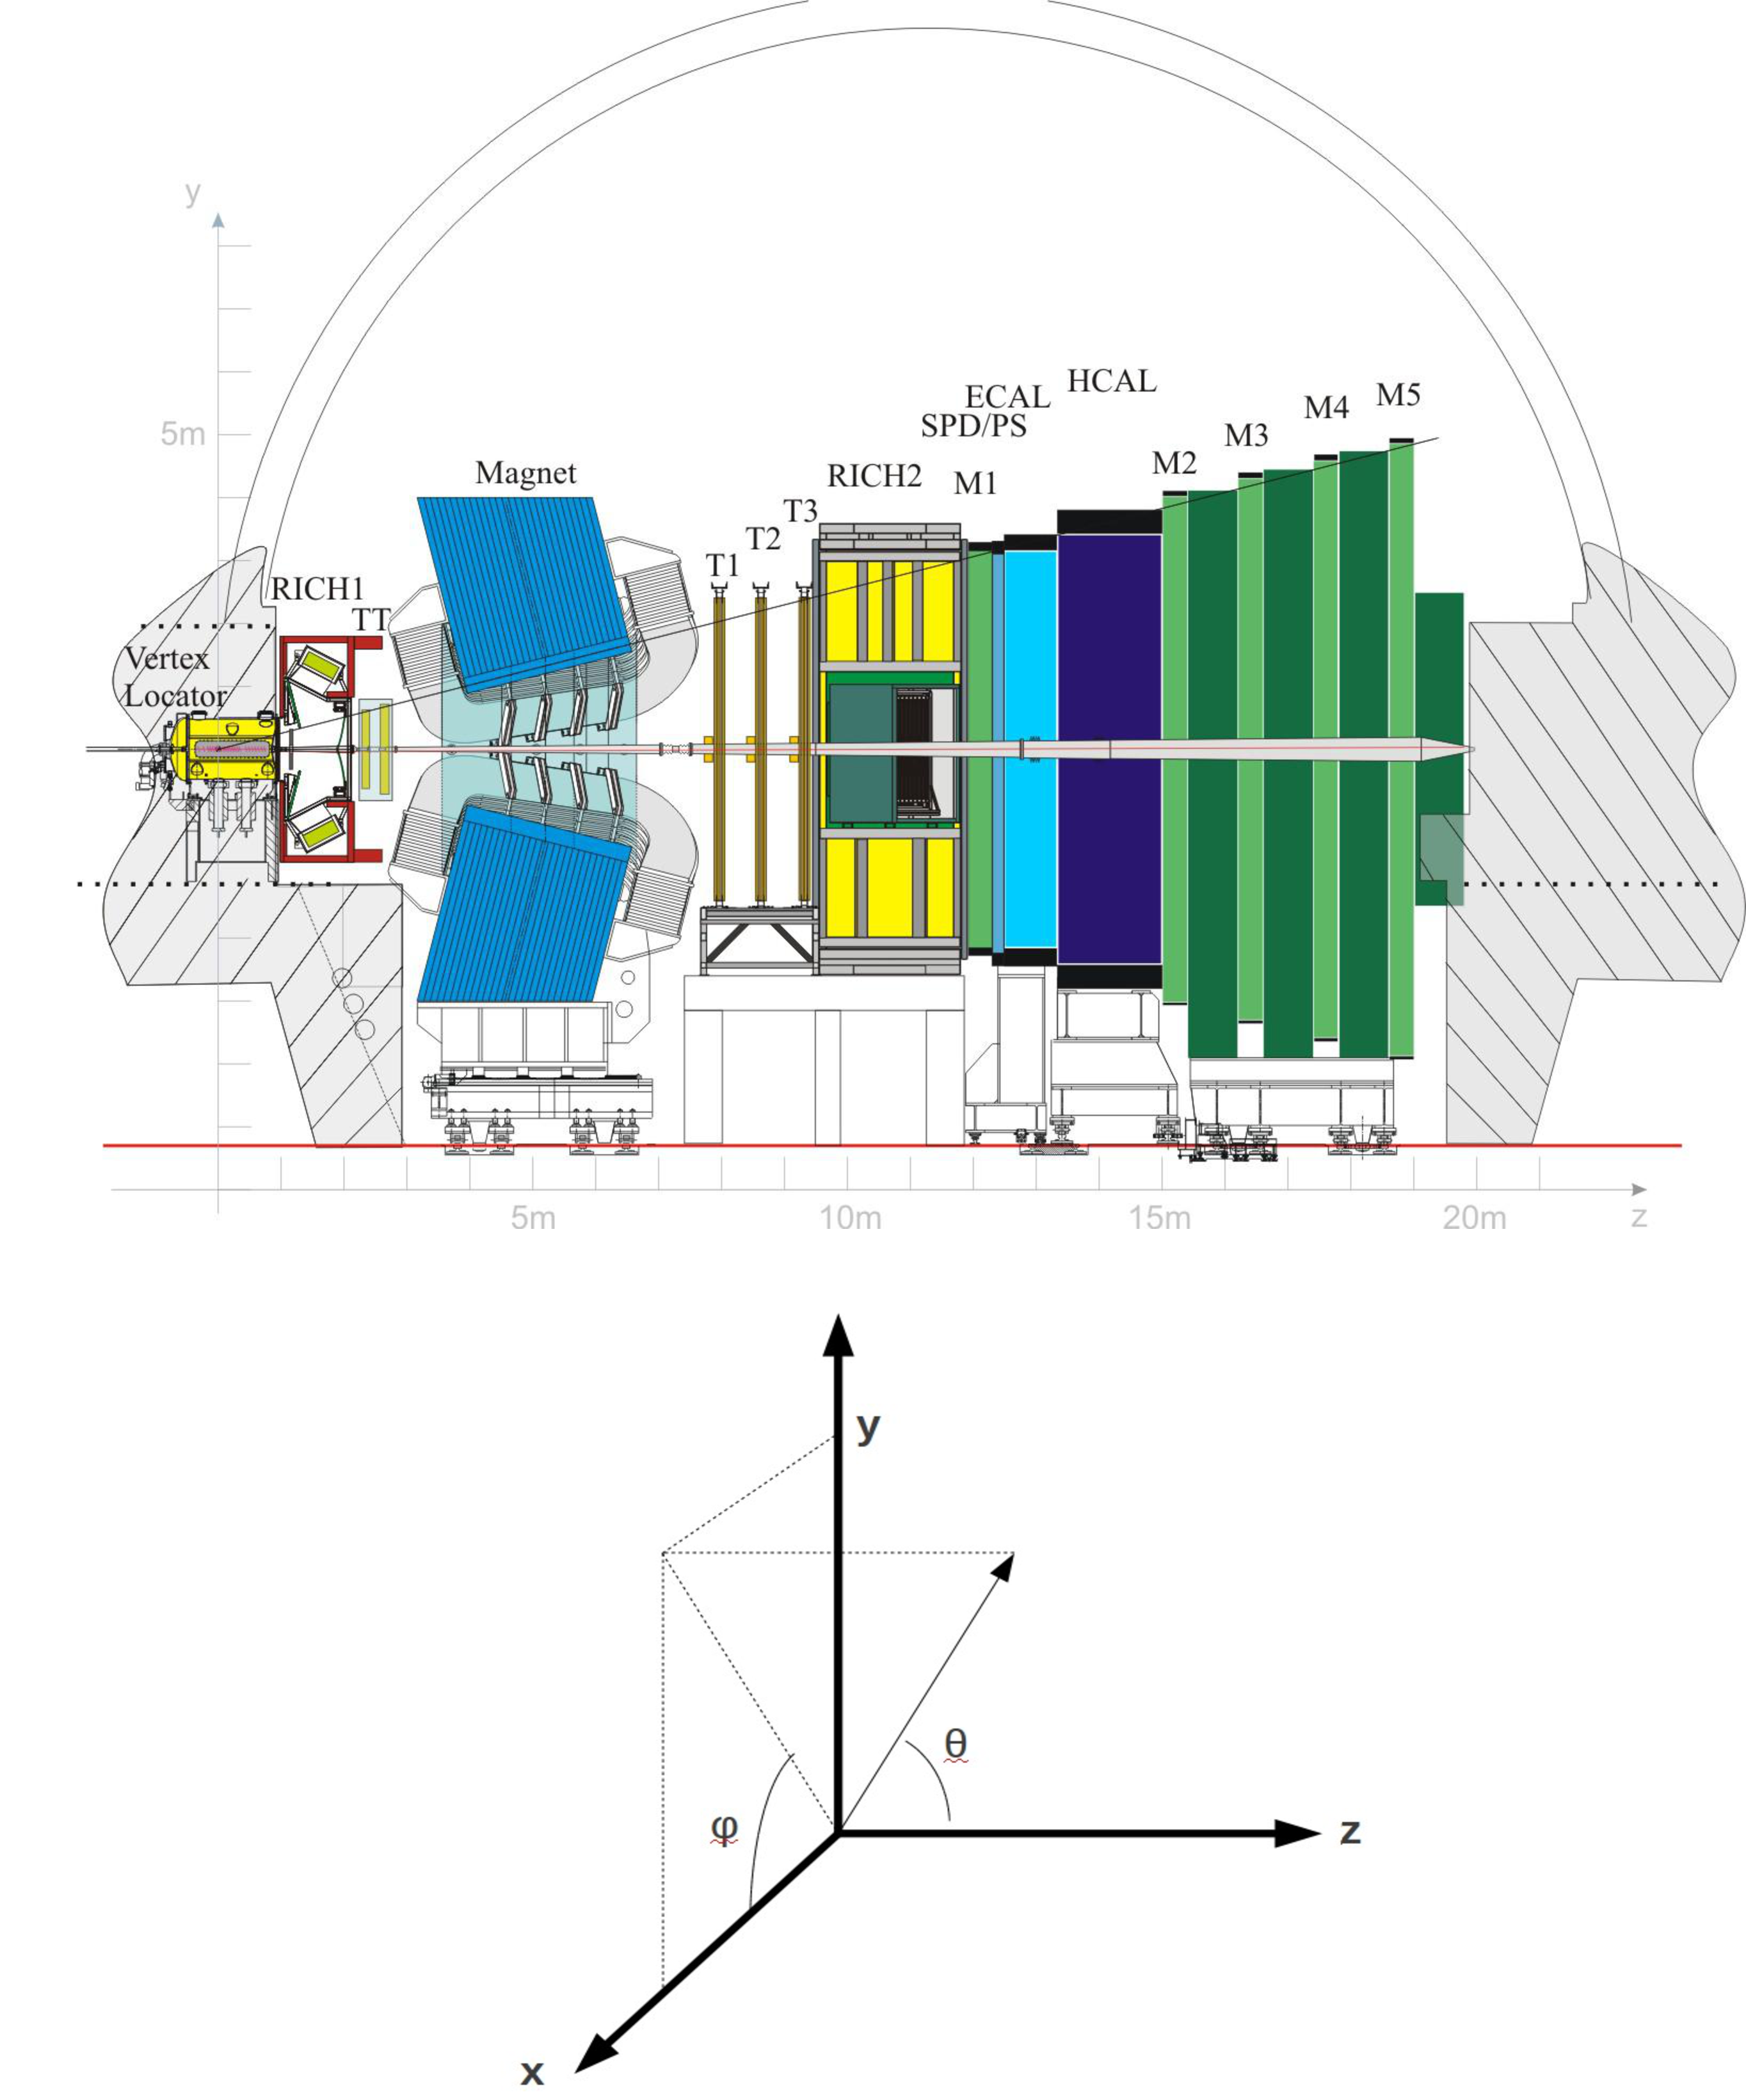
\includegraphics[width=\textwidth]{detectordiagco.pdf}
  \caption{ A schematic diagram of the \lhcb detector and all its components, along with a diagram of the coordinate system used.}
  \label{fig:detectdiag}
\end{figure}
\begin{figure}[h]
  \centering
  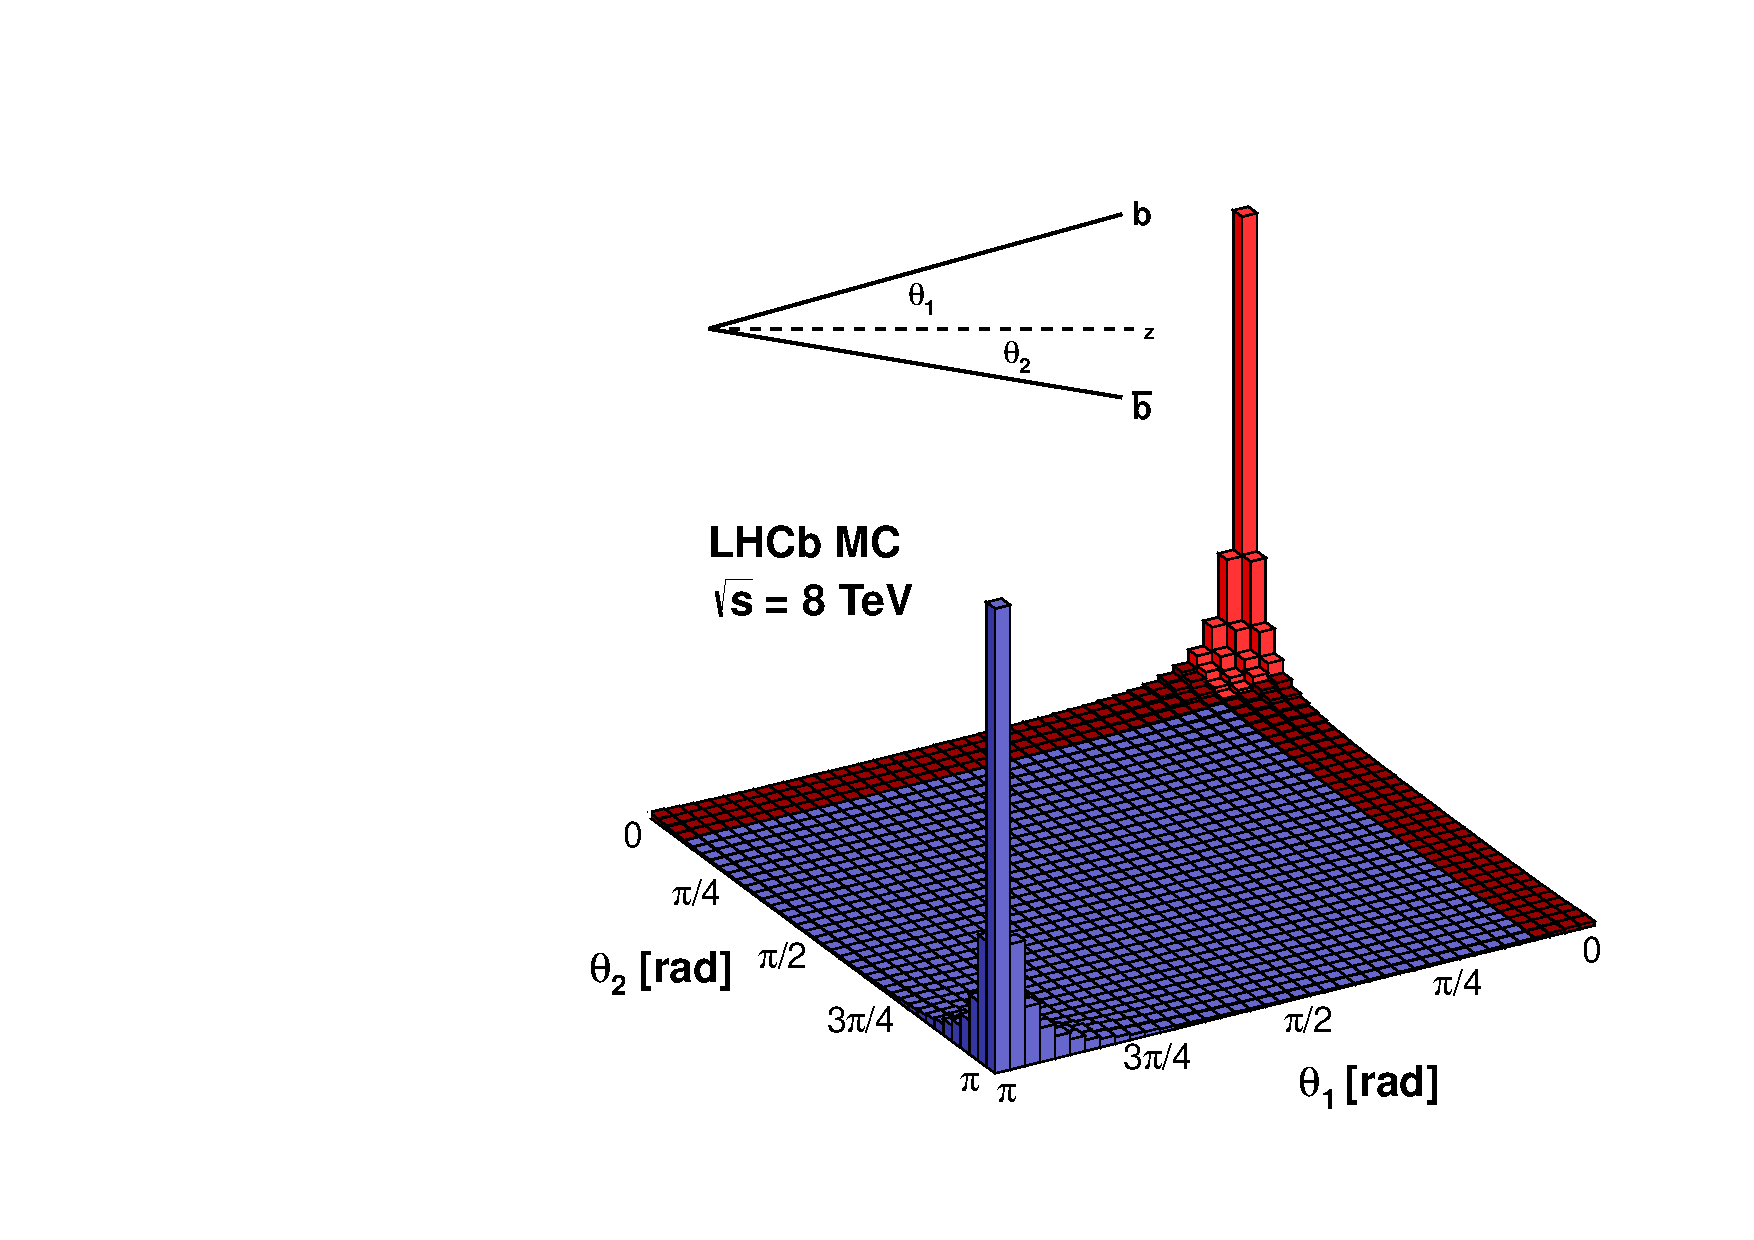
\includegraphics[width=0.5\textwidth]{08_rad_acc_scheme_right.pdf}
  \caption{A diagram showing the angular distribution of $b \bar{b}$ pair production at 8TeV}
  \label{fig:bbarprod}
\end{figure}
\subsection{Tracking}
\label{sec:Tracking}
The objective of any particle physics tracking system is to provide positional information on the path taken by charged particles.  At all collider based experiments the paths of charged particles are curved by a magnetic field to distinguish positive and negatively charged particles, measure momentum and also aid particle identification.  At \lhcb this is performed by a warm dipole magnet, which is subject to a polarity reversal periodically to remove charge specific systematic uncertainties.

The first stage of the \lhcb tracking system is the Vertex Locator (VELO).  When a \Bd meson is created it will travel a measurable distance before it decays.  As the \Bd is neutral it leaves no track, therefore there is a secondary (or displaced) vertex present in the decay.  This is also the case for many other mesons containing b and c quarks.  As these make up such a large section of the \lhcb phyiscs programme, the VELO was developed to detect these secondary vertices.

The VELO consists of several semi-circular silicon sensors which are placed transverse to the beam pipe, with the beam pipe passing through the centre.  A diagram of this is shown in Figure \ref{fig:VELO}.  As shown in Figure \ref{fig:detectdiag} these are positioned upstream of any other detector component as close as possible to the interaction region.  There are two types of sensors, one which provides radial position information of tracks and one which provides azimuthal $(\phi)$ position information.  These work in tandem to provide an optimal track resolution of $4\mu m$ \cite{Aaij:1978280}, which is the best of any tracking system at the LHC.
\begin{figure}
  \centering
  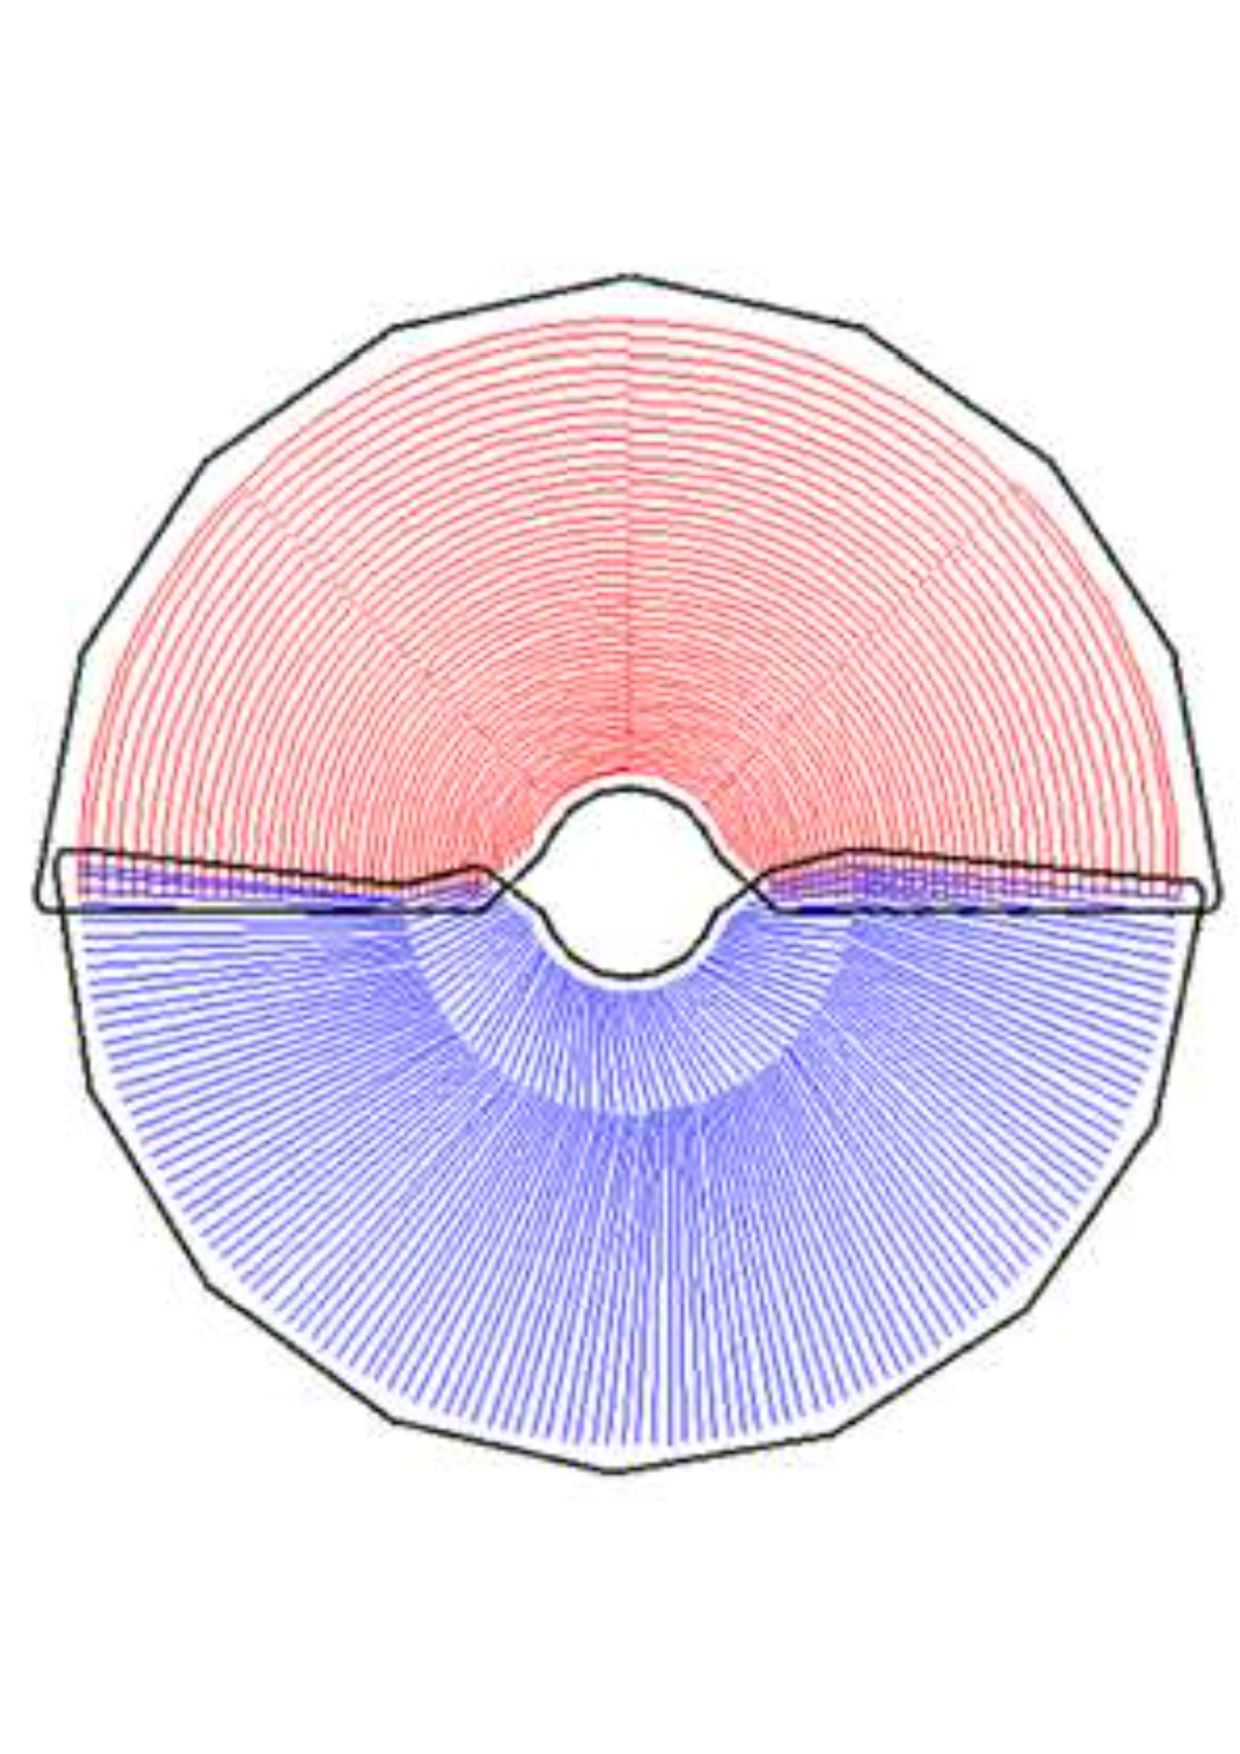
\includegraphics[width=0.5\textwidth]{VELO.pdf}
  \caption{A diagram showing half of each type of VELO sensor in the x,y plance.  The blue sensor provides azimuthal position information and the red sensor provides radial position information.}
  \label{fig:VELO}
\end{figure}

 In one year of running the VELO receives a 1MeV neutron equivalent fluence of $1.3\times10^{14} neq/cm^2$ which makes radiation hardness a challenge \cite{Alves:1129809}.  To keep this fluence to a minimum, the VELO is mechanically moved further away from the beam pipe whilst the LHC is still filling.  During this stage no physics data can be taken, therefore the VELO would be undergoing irradiation for no gain in physics data.

 The next stage of the \lhcb tracking system is positioned just upstream of the dipole magnet, denoted ``TT'' in Figure \ref{fig:detectdiag}.  This also makes use of silicon microstrips to give a positional resolution of $52.6 \mu m$, as measured in run I data \cite{Aaij:1978280}.

The final stage of the tracking system is positioned downstream of the dipole magnet, which is actually three seperate tracking stations labelled T1,T2 and T3 in Figure \ref{fig:detectdiag}.  The inner areas of these tracking stations are silicon microstrips which provide very similar spatial resolution to the TT.  As silicon microstrips are very expensive, the outer areas of the downstream tracking stations are straw tube trackers.  These provide a spatial resolution of $205 \mu m$ \cite{Aaij:1978280}.

 
\subsection{Calorimetry}
\label{sec:Calorimetry}
The role of calorimetry in HEP experiments is predominantly to measure the energy of particles.  However they also play a role in particle identification and, particularly at the LHC, a role in triggering.

The electromagentic calorimeter used by \lhcb is a tried and tested shashlik sampling calorimeter.  It consists of 66 separate layers, each consisting of 2mm of lead and 4mm of plastic scintillator.  This amounts to 25 radiation lengths of material \footnote{ A radiation length is defined as the length of material required to reduce the energy of an incident electron to $\frac{1}{e}$ of its incident energy}.  The role of the lead is to induce an electromagnetic shower as quickly as possible and stop the incident particle within a short distance.  The role of the scintillator is to then measure the energy contained in the EM shower.

The light from the plastic scintillator is transported to photo multiplier tubes by wavelength shifting fibres.  These change the wavelength of the light from the plastic scintillator to a wavelength compatible with the sensitive region of the photo multiplier tubes.  The signal from the PMTs is then proportional to the energy of the incident particle, so the energy of the incident particle can be inferred.

\subsection{Particle Identification}
\label{sec:Particle Identification}
A large section of the \lhcb physics programme relies on the excellent particle identification (PID) ability of the \lhcb detector.  There are many analyses that would not be possible if pions, kaons and protons could not be separated cleanly. A good example of this is the observation of a pentaquark like state \cite{LHCb-PAPER-2015-029}.

The PID performance of the \lhcb detector is largely due to the presence of two ring imaging chernkov detectors (RICH1 and RICH2 in Figure \ref{fig:detectdiag}).  When a charged particle travels faster than the speed of light in a medium it will emit photons at an angle $\theta$ relative to the momentum direction of the charged particle.  The angle at which these photons are radiated is given by,
\begin{equation}
  cos(\theta)=\frac{1}{n\beta}=\frac{E}{np}=\frac{\sqrt{p^2+m^2}}{np}
\end{equation}
where $n$ is the refractive index of the medium and $p$,$E$ and $m$ are the momentum, energy and mass of the charged particle respectively.  The RICH1 detector is filled with $C_4F_{10}$ and RICH2 is filled with $CF_4$.  The refractive index of these media has been measured very accurately \cite{LHCb-DP-2012-003}.

The RICH system measures the angle $\theta$ of cherenkov photons and the momentum of the charged particles can be measured independently of the RICH system with the curvature of the charged tracks.  By combining these measurements, with the knowledge of the refractive index of the medium, one can determine the mass of the charged particle.  It can be determined with sufficient precision to identify the particle.

The performance of the RICH detector varies as a function of charged particle momentum.  During run I, for a momentum-averaged Kaon efficiency of $95\%$, a $10\%$ pion mis-identification rate was observed.  This means $95\%$ of kaons can be correctly identified as kaons whilst only $10\%$ of pions are mis-identified as kaons\cite{Aaij:1978280}.

\subsection{Trigger}
\label{sec:Trigger}
The role of a trigger in a HEP experiment is to decide which events are worth recording.  At the LHC, proton bunches arrive at the interaction point every 25ns therefore collisions happen at a rate of 40MHz.  It is impossible to process and record every single bunch crossing at this rate.  Also, it would not be useful as only a fraction of the inelastic pp interactions that take place at \lhcb produce heavy quark falvours of interest.

The \lhcb trigger system is comprised of 2 distinct levels.  The first level is the L0 trigger, which is entirely implemented in hardware using field programmable gate arrays (FPGAs).  The role of the L0 trigger is to reduce the rate of events from 40MHz to 1.1MHz of potentially useful events.  As these decisions have to be made at such a high rate, only information from the calorimeters and muon system are used in the L0 trigger.

The next stage is the High Level Trigger (HLT), which is an entirely software based trigger that makes use of a computing farm with 26000 processor cores.  The HLT reduces the overall event rate to 3kHz.  However, this is split into two sub-triggers; the HLT1 and HLT2.

The HLT1 reduces the 1.1MHz input rate to 43kHz by partially reconstructing the event.  In addition to the calorimeter and muon information, the information from the VELO and tracking systems is used.  Simple selection criteria based on the information from these sub detectors can then be applied.

Now that the rate is reduced to 43kHz, the HLT2 can perform a full event reconstruction and apply more complete selection critera.  These involve the information from all sub detectors and are often based on topological multivariate requirements \cite{BBDT}.  The rate of events passing the HLT2 is 3kHz, therefore the \lhcb trigger system has reduced the event rate by four orders of magnitude from 40MHz to 3kHz.


\clearpage
